%; whizzy chapter
% -initex iniptex -latex platex -format platex -bibtex jbibtex -fmt fmt
% $B0J>e(B whizzytex $B$r;HMQ$9$k>l9g$N@_Dj!#(B

%     Tokyo Debian Meeting resources
%     Copyright (C) 2011 Junichi Uekawa
%     Copyright (C) 2011 Nobuhiro Iwamatsu

%     This program is free software; you can redistribute it and/or modify
%     it under the terms of the GNU General Public License as published by
%     the Free Software Foundation; either version 2 of the License, or
%     (at your option) any later version.

%     This program is distributed in the hope that it will be useful,
%     but WITHOUT ANY WARRANTY; without even the implied warranty of
%     MERCHANTABILITY or FITNESS FOR A PARTICULAR PURPOSE.  See the
%     GNU General Public License for more details.

%     You should have received a copy of the GNU General Public License
%     along with this program; if not, write to the Free Software
%     Foundation, Inc., 51 Franklin St, Fifth Floor, Boston, MA  02110-1301 USA

%  preview (shell-command (concat "evince " (replace-regexp-in-string "tex$" "pdf"(buffer-file-name)) "&"))
% $B2hA|%U%!%$%k$r=hM}$9$k$?$a$K$O(Bebb$B$rMxMQ$7$F(Bboundingbox$B$r:n@.!#(B
%(shell-command "cd image201201; ebb *.png")

%%$B$3$3$+$i%X%C%@3+;O!#(B

\documentclass[mingoth,a4paper]{jsarticle}
\usepackage{monthlyreport}

% $BF|IU$rDj5A$9$k!"Kh7nJQ$o$j$^$9!#(B
\newcommand{\debmtgyear}{2012}
\newcommand{\debmtgmonth}{2}
\newcommand{\debmtgdate}{18}
% (+ (* (- 2012 2005) 12) 1 -1) started from zero
\newcommand{\debmtgnumber}{85}

\begin{document}

\begin{titlepage}
\thispagestyle{empty}
% $B%?%$%H%k%Z!<%8(B:$BJT=8I,MW$JItJ,$O:G=i$N%^%/%m$KHt$P$9$3$H(B

\vspace*{-2cm}
$BBh(B\debmtgnumber{}$B2s(B $BEl5~%(%j%"(B Debian $BJY6/2q;qNA(B\\
\hspace*{-2cm}
\includegraphics[width=210mm]{image201003/debsen.eps}\\
\hfill{}\debmtgyear{}$BG/(B\debmtgmonth{}$B7n(B\debmtgdate{}$BF|(B

% $B$3$3$O%"%C%W%G!<%H$9$k$3$H(B
% $BA43QJ8;z$K$7$J$$$H%U%)%s%H$N%5%$%:$,9g$o$J$$$N$GCm0U(B
\rotatebox{10}{\fontsize{23}{23} {\gt $BFC=8(B1: Debian$B3+H/<T$N(BKDE$B4D6-$"$l$3$l(B}}

\rotatebox{10}{\fontsize{23}{23} {\gt $BFC=8(B2: $B7n4)(BDebhelper}}

\rotatebox{10}{\fontsize{23}{23} {\gt $BFC=8(B3: cmake}}
\vspace*{-2cm}
\hfill{}
\includegraphics[height=6cm]{image200502/openlogo-nd.eps}
\end{titlepage}

\dancersection{Introduction}{$BLnEg!!5.1Q(B}

\begin{multicols}{2}
 

 $B:#7n$N(BDebian$BJY6/2q$X$h$&$3$=!#$3$l$+$i(BDebian$B$N@$3&$K$"$7$rF'$_F~$l$k$H(B
 $B$$$&J}$b!"$9$G$K$I$C$W$j$H$D$+$C$F$$$k$H$$$&J}$b!"7n$K0l2s(BDebian$B$K$D$$(B
 $B$F8l$j$^$;$s$+!)(B

 Debian$BJY6/2q$NL\E*$O2<5-$G$9!#(B

 \begin{itemize}
 \item \underline{Debian Developer} ($B3+H/<T(B)$B$N0i@.!#(B
 \item $BF|K\8l$G$N!V(B\underline{$B3+H/$K4X$9$k>pJs(B}$B!W$r@0M}$7$F$^$H$a!"%"%C%W%G!<%H$9$k!#(B
 \item \underline{$B>l(B}$B$NDs6!!#(B
 \begin{itemize}
  \item $BIaCJ$P$i$P$i$J>l=j$K$$$k?M!9$,(B face-to-face $B$G=P2q$($k>l$rDs6!(B
	$B$9$k!#(B
  \item Debian $B$N$?$a$K$J$k$3$H$r8l$k>l$rDs6!$9$k!#(B
  \item Debian$B$K$D$$$F8l$k>l$rDs6!$9$k!#(B
 \end{itemize}
 \end{itemize}		

 Debian$B$NJY6/2q$H$$$&$3$H$G5f6KE*$K$O;22C<TA40w$,(BDebian Package$B$r$,$j$,$j(B
 $B$H:n$k%"%/%F%#%V$J3+H/<T$K$J$C$?;Q$rLQA[$7$F$$$^$9!#>pJs$N6&M-!&3hMQ$rDL$7(B
 $B$F(B Debian$B$N:#8e$NG=F0E*$JE83+$X$NEZBf$H$7$F!"!V>l!W$H$7$F$N6u4V$rDs6!$9(B
 $B$k$N$,L\E*$G$9!#(B

\end{multicols}

\newpage

\begin{minipage}[b]{0.2\hsize}
 \definecolor{titleback}{gray}{0.9}
 \colorbox{titleback}{\rotatebox{90}{\fontsize{80}{80} {\gt $B%G%S%"%sJY6/2q(B} }}
\end{minipage}
\begin{minipage}[b]{0.8\hsize}
\hrule
\vspace{2mm}
\hrule
\begin{multicols}{2}
\tableofcontents
\end{multicols}
\vspace{2mm}
\hrule
\end{minipage}

\dancersection{$B;vA02]Bj(B}{$BLnEg(B $B5.1Q(B}

$B:#2s$N;vA02]Bj$O0J2<$G$9(B:
\begin{enumerate}
 \item $B3'$5$s$N(BDebian desktop$B4D6-$H!"MxMQ$K$"$?$C$F2?$+9)IW$,$"$l$P(B200$BJ8;z0JFb$G%"%T!<%k$/$@$5$$!#(B(contrib$BL\I8(B/$BL$Mh;X8~$J%"%T!<%k$O$5$i$K@d;?4?7^!K(B
\end{enumerate}
$B$3$N2]Bj$KBP$7$FDs=P$$$?$@$$$?FbMF$O0J2<$G$9!#(B
\begin{multicols}{2}
{\small
\begin{prework}{ 鈴木崇文 }

gnomeでdesktopを利用しています。
工夫というほどではないですが、便利なツールとしてKDE系のアプリやEBViewを使っています。
リモートデスクトップ(RDP) & VNC 用には、KRDC を使い、スクリーンショット用には KSnapshot を使っています。
あとは英辞郎を購入して、EBViewでいつでも翻訳できるようにしています。
\end{prework}

\begin{prework}{ dictoss(杉本 典充) }

低性能マシンはstartx+icewm、中高性能マシンはgdm+xfce4かgnomeと使い分けています。KDEは最近使ってないです。(KDEは重そうなイメージがある)
カスタマイズしているのは、ページャの個数を6つに増やしている、複数のターミナルを重ならないように同時起動するシェルスクリプトを作り一発で画面をターミナルで埋め尽くせるようにしています。(昔タイル型ウィンドウマネージャ使えばいいのに、とか突っ込まれました)
\end{prework}

\begin{prework}{ yamamoto }

メインに使っているのは、録画サーバも兼ねた Debian squeeze (amd64) です。
外出時は気分次第で、sid の i386 ネットブックと sid の amd64 ノート PC を選んでいます。
どれも、特に何の変てつもない、ただの KDE 環境です。

デスクトップとしての見た目は、壁紙すらデフォルトのままで、改造してませんが、機体としては家の LAN にぶら下がったマシン間を「何か(?)」が行き来する、魔改造スクリプトがいくつか仕込んであり、ものぐさな私にはとっても快適です。
\end{prework}

\begin{prework}{ 野島 貴英 }

GNOME 3.2.2をDebianで利用しています。unstableではもの足りず、experimentalからupgradeして引っ張ってきてます。特にクールなカスタマイズは何もしてないですが、gnome-shellがjavascriptなど解釈できるということから、将来ちょっとしたガジェットぐらい作ってみたいなーと思うこの頃です。あと、gxconsole( \url{http://gnomefiles.org/content/show.php/gxconsole?content=132145} )がGNOME3.2.2になっても、やっぱり欲しかったので、GNOME 3.2.2用に移植したい...
\end{prework}

\begin{prework}{ 日比野 啓 }

普段はタイル型ウィンドウマネージャの XMonad を使っています。
マルチディスプレイに対するサポートが使いやすくてプレゼンのときにも便利で気にいっています。
最近、趣味のプログラミングのメインで使っている言語が Haskell なので、
Haskellでカスタマイズできることも魅力です。
gnome-session との組合せも使ってみましたが、なぜか sid ではうまく動かなくて残念。
あと、画面の上下が狭くなるのが嫌なので、なんとかする方法が知りたい。

\end{prework}

}
\end{multicols}

\dancersection{$B:G6a$N(BDebian$B4XO"$N%_!<%F%#%s%0Js9p(B}{$BLnEg!!5.1Q(B}
\subsection{$BEl5~%(%j%"(BDebian$BJY6/2q(B84$B2sL\Js9p(B}

% (query-replace-regexp "<.*?>" "")
% (query-replace-regexp "^[	 ]\+" "")

  1$B7n$NEl5~%(%j%"(BDebian$BJY6/2q$O5W$7$V$j$K$"$s$5$s$V$k2.7&$K$F9T$o$l$^$7$?!#(B
$B>e@n$5$s$+$i!"(BDebian$BJY6/2qM=Ls%7%9%F%`$K4X$9$k@H<e@-$H9M;!!"$^$?!"(BDebian$B$N(B
$B;H$($k(BVPS$B$K4X$9$kH/I=!"4d>>$5$s$+$i(BDebian$B$r$D$+$C$?(Btwitter$BO"7H$K$D$$$FH/I=(B
$B$,$"$j$^$7$?!#$^$?91Nc$N7n4)(BDebhelper$B$O;3ED$5$s$K$h$jH/I=$,9T$o$l!"(Bdh$B%3%^%s%I(B
$B$^$o$j$r$5$i$K?<KY$j$7$?7o$H!"(Bdh\_builddeb$B%3%^%s%I$K4X$7$FH/I=$,9T$o$l$^$7$?!#(B

$B!!:#8e$^$9$^$9(BWEB$B%7%9%F%`MQES$K$b(BDebian$B$O;H$o$l$F$$$/$H;W$$$^$9!#$3$N$"$?$j$r(B
$B0U<1$7$?H/I=$,B?$+$C$?$N$,0u>]E*$G$7$?!#(B

\dancersection{Debian Trivia Quiz}{$BLnEg(B $B5.1Q(B}

$B$H$3$m$G!"$_$J$5$s(B Debian $B4XO"$NOCBj$K$*$$$D$$$F$$$^$9$+!)(BDebian$B4XO"$NOC(B
$BBj$O%a!<%j%s%0%j%9%H$r$h$s$G$$$k$HDI@W$G$-$^$9!#$?$@$h$s$G$$$k$@$1$G$O$O(B
$B$j$"$$$,$J$$$N$G!"M}2rEY$N%F%9%H$r$7$^$9!#FC$K0l?M$@$1$G$O0UL#$,$o$+$i$J(B
$B$$$H$3$m$b$"$k$+$bCN$l$^$;$s!#$_$s$J$G0l=o$KFI$s$G$_$^$7$g$&!#(B

$B:#2s$N=PBjHO0O$O(B\url{debian-devel-announce@lists.deban.org} $B$d(B \url{debian-devel@lists.deban.org}$B$KEj9F$5$l$?(B
$BFbMF$H(BDebian Project News$B$+$i$G$9!#(B

\begin{multicols}{2}
% %; whizzy-master ../debianmeetingresume201201.tex
% 以上の設定をしているため、このファイルで M-x whizzytex すると、whizzytexが利用できます。
%

\santaku
{Lenny のセキュリティサポートが終わったのはいつ?}
{2012/02/06}
{2012/02/07}
{2012/02/08}
{A}
{}

\santaku
{2012/01/28 に更新された Squeeze のヴァージョンは?}
{6.0.4}
{6.1.0}
{20120128}
{A}
{}

\santaku
{Debian Game チームが 2/25から2/26まで行うイベントは何か?}
{どれだけの Windows のゲームが Wine 上で動作するか検証するパーティ}
{Debian で提供されているゲームパッケージのスクリーンショットを撮りまくるパーティ}
{Debian で提供されているゲームを48時間連続プレイするパーティ}
{B}
{}

\santaku
{Wheezy で採用される Linux カーネルヴァージョンは?}
{2.6.39}
{3.2}
{4.0}
{B}
{}

\santaku
{pts.debian.org で表示されるようになった情報は?}
{パッケージメンテナが誕生日の日は「おめでとう」と出る。}
{パッケージを乗っ取ろうとしている人の情報}
{パッケージ Transition 情報}
{C}
{}

\santaku
{アクセプトされたDEPは?}
{DEP 3}
{3 DEP }
{DEP DEP DEP}
{A}
{DEP3 は Patch tagging guideline. Debian Enhancement Proposals}



\end{multicols}

%-------------------------------------------------------------------------------
\dancersection{Debian$B3+H/<T$N(BKDE$B4D6-$"$l$3$l(B}{$BLnEg!!5.1Q(B}
%-------------------------------------------------------------------------------

\index{Debian$B$+$$$O$D$7$c$N(BKDE$B$+$s$-$g$&(B@Debian$B3+H/<T$N(BKDE$B4D6-(B}

$B!!:G6a$N(BDebian$B$r$=$N$^$^%$%s%9%H!<%k$9$k$H!"FC$K;XDj$7$J$$>l9g(BGNOME$B$H$$$&(B
$B%G%9%/%H%C%W4D6-$,%$%s%9%H!<%k$5$l$^$9!#$7$+$7$J$,$i!"(BDebian$B$G$O$$$/$D$b(B
$B%G%9%/%H%C%W4D6-$,MQ0U$5$l$F$*$j!"%f!<%6$O<+M3$K$3$l$i$rA*$s$G;H$&$3$H$,(B
$B$G$-$^$9!#%G%9%/%H%C%W4D6-$O%f!<%6$K$H$C$F$O$$$D$b;H$&4D6-$G$9$+$i!"(B
$B$$$m$$$m$H$3$@$o$j$b$"$k$+$H$*$b$$$^$9!#:#2s$O(BKDE$B$H$$$&%G%9%/%H%C%W4D6-$K(B
$B$D$$$F$"$l$3$l8l$j$^$9!#(B

\subsection{$BMxMQ<T$H$7$F$N(BKDE$BF3F~J}K!(B}

$B!!(BDebian$B$N0BDjHG$NMxMQ$r8!F$$7$F$$$F!"(BKDE$B4D6-$r$$$o$f$kMxMQ<T$H$7$F(B
$B;H$&0Y$K%$%s%9%H!<%k$9$k$d$jJ}$K$D$$$F4JC1$K=R$Y$^$9!#(B

\begin{enumerate}
 \item $B0BDjHG$N(BDebian$B$N%$%s%9%H!<%k(BDVD$B$rMQ0U$7$^$9!#(B
 \item $B%$%s%9%H!<%i$N%a%K%e!<2hLL$,=P$^$7$?$i!"(BTAB$B%-!<$r$*$9$H2hLL2<$NJ}$KJT=82DG=$J9T$,8=$l$^$9$N$G!"0J2<$NNc$h$&$K(B''desktop=kde''$B$H$$$&J88@$rDI2C$7$^$9!#$J$*!"F|K\8l(B106$B%-!<%\!<%I$r;H$C$F$$$k>l9g!"%-!<%H%C%W$N9o0u$NDL$j$K(B''=''$B$r2!$7$F$b(B''=''$BJ8;z$,F~NO$G$-$J$$>l9g$,$"$j$^$9$,!"$3$N>l9g$O(B''\verb|^|''$B$N9o0u$N%-!<$r2!$9$H(B''=''$BJ8;z$,F~NO$G$-$^$9!#(B
\begin{commandline}
 /install.amd/vmlinuz vga=788 initrd=/install.amd/initrd.gz --- quiet desktop=kde
\end{commandline}
\begin{figure}[ht]
\begin{center}
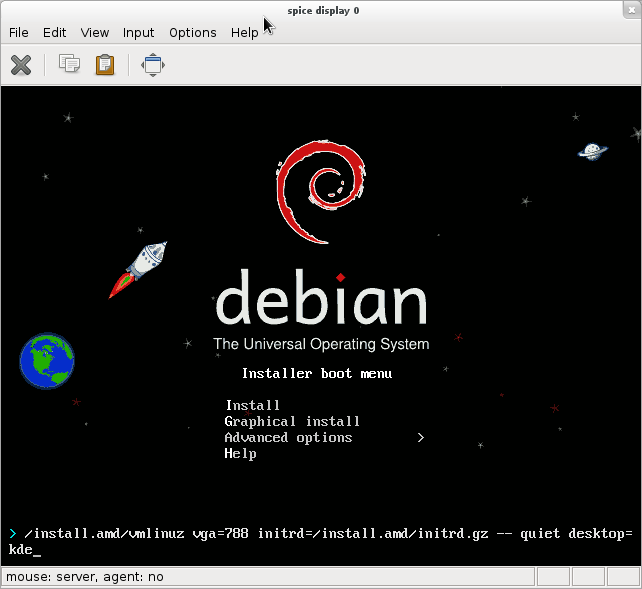
\includegraphics[width=7cm]{image201202/kdedesk/stable-inst-menu.png}
\caption{$B0BDjHG%$%s%9%H!<%k2hLL$G(BTAB$B%-!<$r2!$7$?$H$-$NMM;R(B}
\end{center}
\end{figure}
\item $B$"$H$ODL>o$I$*$j%$%s%9%H!<%k$r9T$$$^$9!#%$%s%9%H!<%k$r?J$a$F$$$/$H!V%=%U%H%&%'%"$NA*Br!W$H$$$&%a%K%e!<$G!V%$%s%9%H!<%k$9$k%=%U%H%&%'%"$NA*Br(B:$B!W$N%a%K%e!<$,8=$l$^$9$N$G!"(B''Debian desktop environment''$B$rA*Br$7$F$*$$$F$/$@$5$$!#(B
\item $B%$%s%9%H!<%k$,40N;$7$^$7$?$i!"%j%V!<%H$r9T$$$^$9!#(B
\item KDE$B4D6-$,5/F0$7$^$9!#(B
\end{enumerate}

$B0J>e$H$J$j$^$9!#4JC1$G$9$M!#(B

\subsection{\label{sec:exp-kde}$B3+H/<T$H$7$F$N(Bexperimental$BHG(BKDE$BF3F~J}K!(B(KVM+spice)}

$B!!El5~%(%j%"(BDebian$BJY6/2q$K$$$i$C$7$c$k$h$&$JJ}!9$K$O!"A0=R$N%$%s%9%H!<%k$H4D6-$G$O(B
$B$-$C$H!V$L$k%2!<!J>P!K!W$J46$8$N$O$:$G$9!#$=$N>l9g!"@'Hs$H$b(B
experimental$BHG$N(BKDE$B4D6-$rMxMQ$$$?$@$-!"(BBTS$B=q$-(B/$B%Q%C%A3+H/(B/$BK]Lu(B/$B%G%P%C%0$J$I$N(B
$B3+H/3hF0$K6P$7$s$G$_$^$7$g$&!#$3$3$G$O!"3+H/<T8~$1(BKDE$B4D6-F3F~$K$D$$$F4JC1$K=R$Y$^$9!#(B

\begin{itemize}
\item $B3+H/<T8~$1$K(Bexperimental$BHGF3F~$rA0Ds$K$7$^$9!#(B
\item $B2>A[4D6-$G$"$k(BKVM$B$rMxMQ$7$F2>A[4D6->e$KF3F~$7$^$9!#$3$l$J$i!"%G%#%9%/%$%a!<%8%U%!%$%k$r$H$C$F$*$1$P!"$&$C$+$j(Baptitude full-upgrade$B$7$FA4$/N)$A>e$,$i$J$/$J$C$F$b$"$C$5$jI|5"$G$-$^$9!#(B
\item $B%5%&%s%I$bM_$7$$$N$G(BVDP$B$K$O(Bspice$B$r;H$$$^$9!#(B
\item $B$$$D$G$b$I$3$G$b3+H/$G$-$k$h$&$K%b%P%$%k4D6-$K9=C[$7$^$9!#(B
\end{itemize}
$B?^(B\ref{fig:kde-env}$B$N(BKDE$B3+H/4D6-$NMQ0U$rA[Dj$7$^$9!#(B

\begin{figure}[ht]
\begin{center}
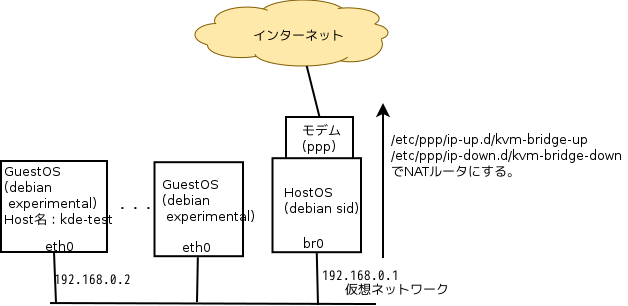
\includegraphics[width=10cm]{image201202/kdedesk/kde-dev-env.png}
\caption{\label{fig:kde-env}KDE$B3+H/4D6-(B}
\end{center}
\end{figure}

$B0J2<$OF3F~$K4X$7$F$NN.$l$G$9!#!J:Y$+$$;v$O3d0&$7$^$9!K(B
\begin{enumerate}
\item HostOS$B$H$J$k(BPC$B$N(BBIOS$B$rA`:n$7$F!"(BCPU$B$N2>A[;Y1g5!9=$N%9%$%C%A$r(BON$B$K$7$F%V!<%H$7$F$*$-$^$9!#(B
\item HostOS$B$K(B\url{http://www.debian.org/CD/netinst}$B$+$iL>;I%5%$%:$N(BCD$B%$%a!<%8$rMn$H$7$FCV$-$^$9!#(B
\item HostOS$B$N(B/etc/network/interfaces$B$K0J2<$NDI5-$r9T$$!"(Bbr0$B$r:n$C$F$*$-$^$9!#(B
\begin{commandline}
# $BDI5-$O$3$3$+$i!#(Baptitude install bridge-utils$B$O$d$C$F$*$/$3$H!#(B
auto br0
iface br0 inet static
        address 192.168.0.1
        netmask 255.255.255.0
        bridge_ports none
        bridge_stp off
        bridge_fd 0
        bridge_maxwait 0
\end{commandline}
\item HostOS$B$N(B/etc/sysctl.d/bridge-filter-workaround.conf$B$r:n$j!"(Bsysctl -p /etc/sysctl.d/bridge-filter-workaround.conf$B$r<B9T$7$F!"(Bbr0$B$N%U%#%k%?$rL58z2=$7$F$*$-$^$9!#(B
\begin{commandline}
# /etc/sysctl.d/bridge-filter-workaround.conf$B$NCf?H(B
net.bridge.bridge-nf-call-ip6tables = 0
net.bridge.bridge-nf-call-iptables = 0
net.bridge.bridge-nf-call-arptables = 0
\end{commandline}
\item HostOS$B$N(B/etc/ppp/ip-up.d/kvm-bridge-up,/etc/ppp/ip-down.d/kvm-bridge-down$B$r:n$C$F$*$-$^$9!#B>$K%U%#%k%?$H$+I,MW$G$"$l$PE,Ev$K$I$&$>!#(B
\begin{commandline}
#!/bin/sh
# /etc/ppp/ip-up.d/kvm-bridge-up$B$NCf?H(B
PATH=/bin:/usr/bin:/sbin:/usr/sbin
CDPATH=
sysctl -w net.ipv4.ip_forward=1
iptables -t nat -A POSTROUTING -o $PPP_IFACE -j MASQUERADE
iptables -A FORWARD -i br0 -o $PPP_IFACE -j ACCEPT
\end{commandline}
\begin{commandline}
#!/bin/sh
# /etc/ppp/ip-down.d/kvm-bridge-down$B$NCf?H(B
#!/bin/sh
PATH=/bin:/usr/bin:/sbin:/usr/sbin
CDPATH=
sysctl -w net.ipv4.ip_forward=0
iptables -t nat -D POSTROUTING -o $PPP_IFACE -j MASQUERADE
iptables -D FORWARD -i br0 -o $PPP_IFACE -j ACCEPT
\end{commandline}
\item HostOS$B$K(Bkvm/libvirt/spice-client-gtk$B%Q%C%1!<%8$rF3F~$7$F$*$-$^$9!#(B
\item HostOS$B$K$F(BGuestOS$BMQ$N(Bkde-test.xml$B$r0J2<$N?w7A$G:n@.$7$F(Bvirsh define kde-test.xml$B$7$F$*$-$^$9!#(B(virt-install$B$O2?8N$+(BSegmentation Fault$B$GMn$A$F$7$^$&$N$G$3$3$G$O;H$$$^$;$s!K(B
\begin{commandline}
<domain type='kvm'>
  <name>kde-test</name>
  <memory>1048576</memory>
  <vcpu>1</vcpu>
  <os>
    <type arch='x86_64' machine='pc-1.0'>hvm</type>
    <boot dev='hd'/>
    <boot dev='cdrom'/>
    <bootmenu enable='yes'/>
  </os>
  <features>
    <acpi/>
    <apic/>
    <pae/>
  </features>
  <clock offset='utc'/>
  <on_poweroff>destroy</on_poweroff>
  <on_reboot>restart</on_reboot>
  <on_crash>restart</on_crash>
  <devices>
    <emulator>/usr/bin/kvm</emulator>
    <disk type='file' device='disk'>
      <driver name='qemu' type='raw' cache='writeback'/>
      <source file='/var/lib/libvirt/images/kde-test.img'/>
      <target dev='vda' bus='virtio'/>
    </disk>
    <disk type='file' device='cdrom'>
      <driver name='qemu' type='raw'/>
<!-- directory of cdimage$B$OE,Ev$KJQ99$/$@$5$$(B -->
      <source file='/directory of cdimage/debian-6.0.4-amd64-businesscard.iso'/>
      <target dev='hdc' bus='ide'/>
      <readonly/>
    </disk>
    <controller type='ide' index='0'/>
    <interface type='bridge'>
<!-- mac$B%"%I%l%9$OE,Ev$KJQ99$/$@$5$$(B -->
      <mac address='52:54:00:31:cd:5a'/>
      <source bridge='br0'/>
      <model type='virtio'/>
    </interface>
    <serial type='pty'>
      <target port='0'/>
    </serial>
    <console type='pty'>
      <target type='serial' port='0'/>
    </console>
    <input type='mouse' bus='ps2'/>
    <graphics type='spice' port='5900' autoport='no'>
      <clipboard copypaste='yes'/>
    </graphics>
    <sound model='ac97'\>
    <video>
      <model type='qxl' vram='9216' heads='1'/>
    </video>
    <memballoon model='virtio'>
    </memballoon>
  </devices>
</domain>
\end{commandline}
\item HostOS$B$G2>A[4D6-MQ$N%G%#%9%/$r(B10GB$B$0$i$$$G:n$C$F$*$-$^$9!#(B
\begin{commandline}
qemu-img create -f raw /var/lib/libvirt/images/kde-test.img 10G
\end{commandline}
\item HostOS$B$G(BKVM$B$r5/F0$7$F!"(Bspice$B%/%i%$%"%s%H$r@\B3$7$^$9!#(B
\begin{commandline}
virsh start kde-test; spicy -h 127.0.0.1 -p 5900 &
\end{commandline}
\item GuestOS$B$N(BDebian$B%$%s%9%H!<%i$,5/F0$7$?$i!"(BTAB$B%-!<$r2!$7!"2hLL2<$K8=$l$?JT=82DG=$J9T$K!"(B''priority=medium''$B$r0J2<$N$h$&$KF~NO$7$F%$%s%9%H!<%k$r3+;O$7$^$9!#(B
\begin{commandline}
 /install.amd/vmlinuz vga=788 initrd=/install.amd/initrd.gz --- quiet priority=medium
\end{commandline}
$B%$%s%9%H!<%kESCf!V(BDebian $B%"!<%+%$%V$N%_%i!<$rA*Br!W$N%a%K%e!<$K$F(B''sid''$B$rA*Br$7!"!V%$%s%9%H!<%k$9$k%3%s%]!<%M%s%H!W$H$7$F!V(Bssh$B%5!<%P!<!W$N$_(B($BB>$OA*Br$7$J$$(B)$B$H$7$^$9!#(B
\item $B%$%s%9%H!<%k$,40N;$9$k$H!"%F%-%9%H%3%s%=!<%k$+$i(BDebian sid$B$J(BGuestOS$B$X%m%0%$%s$G$-$k$h$&$K$J$j$^$9!#(B
\item GuestOS$B$K%m%0%$%s$7$F0J2<$N9T$r(B/etc/apt/source.list$B$XIU$12C$($^$9(B
\begin{commandline}
#$BDI2CFbMF(B
deb http://ftp.jp.debian.org/debian/ experimental main
deb-src http://ftp.jp.debian.org/debian/ experimental main
\end{commandline}
\item GuestOS$B$N(B/etc/apt/preference.d$B$K(BDebian KDE$B%A!<%`@=$N(Bexperimental$B%Q%C%1!<%8MQ(Bpreference$B%U%!%$%k$r%$%s%9%H!<%k$7$^$9!#(B
\begin{commandline}
cd /etc/apt/preference.d && wget http://pkg-kde.alioth.debian.org/files/kde-experimental
\end{commandline}
\item GuestOS$B$G0J2<$r<B9T$7!"(Bexperimental$B$J(BKDE$B4D6-$r0l5$$KF~$l$F$7$^$$$^$9!#(B
\begin{commandline}
aptitude update;aptitude aptitude install task-kde-desktop task-japanese-kde-desktop;aptitude clean
\end{commandline}
\item $B%$%s%9%H!<%k$,=*$o$C$?$i!"(BGuestOS$B$r%j%V!<%H$7$^$9!#(BGuestOS$B$G(BKDE$B$N(Bexperimental$BHG$,5/F0$7!"%0%i%U%#%+%k$J%m%0%$%s2hLL$,8=$l$^$9!#(B
\end{enumerate}

\subsection{Debian$B$H(BKDE$B4D6-$N%P!<%8%g%s(B}

Debian$B$N%P!<%8%g%s$H(BKDE$B$N%P!<%8%g%s$NBP1~$rI=(B\ref{tab:kde-ver}$B$K:\$;$^$9!#(B

\begin{table}[ht]
\begin{center}
\begin{tabular}{|l|l|l|l|l||l|}
\hline 
Debian&stable&testing&unstable&experimental&upstream\\
\hline \hline
KDE &4.4&4.6&4.6&4.7.4&4.8.0\\
\hline
\end{tabular}
\caption{\label{tab:kde-ver}Debian$B$N%P!<%8%g%s$H(BKDE$B$N%P!<%8%g%s(B}
\end{center}
\end{table}

KDE$B$N(Bupstream$B$O(B2012$BG/(B1$B7n(B25$BF|$K(B4.8.0$B$r%j%j!<%9$7$?$P$+$j$J$N$G!"$^$@(B
experimental$B$bDI$$$D$$$F$$$J$$>uBV$G$9!#(B

\subsection{KDE$B4D6-$N3+H/$NFCD'(B}

KDE$B4D6-$N3+H/$O0J2<$N$h$&$JFCD'$,$"$j$^$9!#(B

\begin{enumerate}
\item Qt$B!J%-%e!<%H!K%i%$%V%i%j$r;H$&!#(B
\item C++$B$N%3!<%I$,4pK\(B
\item autotools$B$NBe$o$j$K(Bcmake$B$,;H$o$l$k(B
\end{enumerate}

$B$3$N$?$a!"(BDebian$B$G$O%Q%C%1!<%83+H/$N0Y$K(Bpkg-kde-tools$B%Q%C%1!<%8$,MQ0U$5$l$F$$$^$9!#(B

\subsection{Debian$B$G$N(BKDE$B4D6-$N%Q%C%1!<%83+H/(B}

 Debian$B$G$O(BKDE$B4D6-$N%Q%C%1!<%83+H/MQ$K(Bpkg-kde-tools$B$H$$$&%Q%C%1!<%8$rJL$KMQ0U$7$F$$$^$9!#$3$A$i$rF3F~$9$k$H(BKDE$B4D6-$N%Q%C%1!<%89=C[$N:]$KJXMx$J5!G=$,;H$($k$h$&$K$J$j$^$9!#(B

\begin{table}[ht]
\begin{center}
\begin{tabular}{|l|l|l|l|}
\hline 
$B9`HV(B&$B3HD%$5$l$k$b$N(B&$B3HD%(B&$BHw9M(B\\
\hline
1&dh& --with kde & debhelper$B$K(Bkde$BMQ$N3HD%$r;XDj(B\\
\hline
2&dh\_auto\_*& --buildsystem=kde & dh\_auto\_*$B$,(Bcmake$B$r;H$&$h$&$K$J$k(B\\
\hline
3&CDBS&kde.mk& CDBS$B$G(BKDE$BMQ$N3HD%$,MxMQ$G$-$k$h$&$K$J$k(B\\
\hline
4&$B$=$NB>(B&variables.mk$B$J$I(B& debian/rules$B$NCf$G(B\$(DEB\_CMAKE\_KDE4\_FLAGS)$B$J$I$,;H$($k(B\\
\hline
\end{tabular}
\caption{\label{tab:pkg-kde-tools-inst}pkg-kde-tools$B$r%$%s%9%H!<%k$7$?;~$N3HD%(B}
\end{center}
\end{table}

\subsection{$BD64J0WE*$K(BKDE$BMQ%W%m%0%i%`$N(BDebian$B%Q%C%1!<%8$r:n$C$F$_$k(B}

$B$3$3$G$OD64J0WE*$K(BKDE$BMQ%W%m%0%i%`$N(BDebian$B%Q%C%1!<%8$r:n$C$F$_$^$9!#(B

$B$^$:!";vA0=`Hw$H$7$F!"(B

\begin{itemize}
\item$B!!4D6-$O(B\ref{sec:exp-kde}$B>O$N(Bexperimental$B4D6-$rMQ0U$/$@$5$$!#(B
\item  $B$A$g$HMpK=$G$9$,!"(Baptitude build-dep kdeutils$B$7$F$*$$$F(BKDE$B%Q%C%1!<%83+H/$KI,MW$J%Q%C%1!<%8$rF3F~$7$F$*$-$^$9!#(B
\end{itemize}

$B<!$K(Bkhello-1.0.0/$B$J$k%G%#%l%/%H%j$K(B\url{http://techbase.kde.org/Development/Tutorials/First_program}$B$K$"$k!"(Bmain.cpp$B$H(BCMakeLists.txt$B$rG[CV$7$^$9!#(B

\begin{commandline}
$ cd khello-1.0.0
$ ls 
CMakeLists.txt main.cpp
$
\end{commandline}
% $ 

$B<!$K!"%*%j%8%J%k$N(Btar.gz$B%"!<%+%$%V$r:n@.$7$F$*$-$^$9!#(B

\begin{commandline}
$ cd ..
$ tar czf khello_1.0.0.orig.tar.gz khello-1.0.0
$ ls -F 
khello-1.0.0/  khello_1.0.0.orig.tar.gz
$
\end{commandline}

dh\_make $B$r;H$C$F(Bdebian/$B%G%#%l%/%H%j$r;E9~$_$^$9!#$"$H$O(Brules$B%U%!%$%k0J30(B
$B$$$D$bDL$j!"%Q%C%1!<%8$r:n@.$9$k$h$&$K%U%!%$%k$r:n@.$7$F$*$-$^$9!#(B

\begin{commandline}
$ cd khello-1.0.0/debian
$ ls -F
README.Debian  changelog  control    docs   source/
README.source  compat     copyright  rules
$ 
\end{commandline}
% $

pkg-kde-tools$B%Q%C%1!<%8$rMxMQ$9$k(Brules$B%U%!%$%k$r5-:\$7$^$9!#(B

\begin{commandline}
# pkg-kde-tools$B$r;H$C$?(BKDE$B3+H/MQ(Bdebian/rules$B%U%!%$%k$NCf?H!#(B

%:
       dh $@ --with kde
\end{commandline}
%$

$B$"$H$O!"(Bdpkg-buildpackage -uc -us -rfakeroot$B$r<B9T$7$F%S%k%I$7$^$9!#(B

\begin{commandline}
$ dpkg-buildpackage -us -uc -rfakeroot
dpkg-buildpackage: source package khello
...$BCfN,(B...
dpkg-source: info: building khello in khello_1.0.0-1.debian.tar.gz
dpkg-source: info: building khello in khello_1.0.0-1.dsc
 debian/rules build
dh build  --with kde
   dh_testdir
   dh_auto_configure --buildsystem=kde
-- The C compiler identification is GNU
-- The CXX compiler identification is GNU
...$BCfN,(B...
\end{commandline}
%$

 $BL5;v!"(B--buildsystem=kde$B$,MxMQ$5$l!"(Bcmake$B$,<B9T$5$l$F$$$^$9!#(B

 $B$7$P$i$/BT$D$HL5;v$K(Bkhello\_1.0.0-1\_amd64.deb$B$J$I$,=PMh>e$,$j$^$9!#(B

 $B$[$i!"(Bpkg-kde-tools$B$N$*$+$2$G%Q%C%1!<%83+H/$b4JC1$G$7$g(B?$B$G$7$g!)(B

\subsection{$B$*$o$j$K(B}

 $B:#2s$O!"(BDebian$B3+H/<T$N0Y$N(BKDE$B4D6-$N9=C[$H!"4JC1$J%Q%C%1!<%8:n@.$K$D$$$F!"(B
$B0lDL$j5-:\$7$F$_$^$7$?!#$3$l$r5!$K!"(BKDE$B4D6-$K4X$9$k3+H/$r$5$l$kJ}$,A}$($k$H(B
$B$&$l$7$$$H;W$C$F$$$^$9!#(B

\subsection{$B;29MJ88%(B}

\begin{itemize}
\item \url{http://pkg-kde.alioth.debian.org/} Debian KDE Team$B$N%[!<%`%Z!<%8!#(B
\item \url{http://techbase.kde.org} KDE Techbase
\item \url{http://kde.org/} KDE$BK\2H(B
\end{itemize}

%-------------------------------------------------------------------------------
\dancersection{$B7n4)(BDebhelper}{$B;3K\(B}
%-------------------------------------------------------------------------------

%-------------------------------------------------------------------------------
\dancersection{cmake$B;H$C$F$_$k(B}{$BLnEg(B $B5.1Q(B}
%-------------------------------------------------------------------------------

\index{cmake$B$D$+$C$F$_$k(B@cmake$B;H$C$F$_$k(B}

\subsection{cmake$B$H$O(B}

KDE$B4D6-$N3+H/$K;H$o$l$F$$$k%D!<%k$K(Bcmake$B$,$"$j$^$9!#$3$l$O=>Mh$N(Bautotools
$B$N$h$&$J$b$N$G$9$,!"<!$K=R$Y$kBeI=E*$JFCD'$,$"$j$^$9!#(B

\subsubsection{$B%P%$%J%j$N%W%m%0%i%`$G$"$k(B}

$B!!(Bautotools$B$O!"$4B8CN$NDL$j!"Cf$O(Bsh$B%9%/%j%W%H$H$J$C$F$$$^$9!#$3$l$O(B
/bin/sh$B$r4pK\%3%^%s%I$H$7$F;}$D=>Mh$N(BUNIX$B7O$N(BOS$B$G;H$&$J$iHs>o$KET9g$,$h(B
$B$$$N$G$9$,!"$=$b$=$b(B/bin/sh$B$r;}$?$J$$%7%9%F%`$N85$GMxMQ$7$h$&$H$9$k$H(B
$BF0:n$G$-$^$;$s!#$3$l$G$O!"I8=`E*$J(BC$B%W%m%0%i%`$r%3%s%Q%$%k=PMh$k4D6-(B
$B$J$N$K!"(B/bin/sh$B$,L5$$$H$$$&K\<A$G$O$J$$M}M3$G0\?"@-$rB;$J$&$N$O$A$g$C$H(B
$B;DG0$G$9!#(B

 cmake$B$O%P%$%J%j$N%W%m%0%i%`$J$N$G!"%3%^%s%IC1BN$GF0:n$9$k$3$H$,$G$-!"(B
/bin/sh$B$J$I(BUNIX$B$N%3%^%s%I$,L5$$>l=j$G$bLdBj$J$/F0:n$G$-$^$9!#(B

\subsubsection{$BMM!9$J%W%i%C%H%U%)!<%`MQ$N9=C[%7%9%F%`$KBP1~$G$-$k(B}

$B!!(Bautotools$B$O(Bmake$B$KFC2=$7$?%D!<%k$H$J$j$^$9!#$3$3$G!"$=$b$=$b(BMakefile$B$,(B
$B0lHLE*$G$O$J$$3+H/4D6-!JNc!'(BMicrosoft Visual Studio$BEy$NMM!9$J(BIDE)$B$N>l9g!"(B
Makefile$B$h$j$b(B.proj$B%U%!%$%k$r@8@.$G$-$?J}$,$h$jET9g$,$h$+$C$?$j$7$^$9!#(B

  cmake$B$O0lK\$N(BCMakeLists.txt$B$rMQ0U$9$k$@$1$G!"(BMakefile$B$d!"(BIDE$B4D6-MQ(B
$B$N(B.proj$B%U%!%$%k$r@8@.$G$-$?$j$9$kG=NO$,$"$j$^$9!#$3$N0Y!"(Bautotools$B$r(B
$BMxMQ$7$?%=!<%9%Q%C%1!<%8$N$h$&$K!"(BMakefile.am$B$H(B.proj$B%U%!%$%k$rJL!9$K(B
$B=$@5$7$F(BUNIX/Windows$B4V$N0\?"@-$rJ]$D$H$$$&$h$&$J:n6H$+$i3+H/<T$O3+J|(B
$B$5$l$^$9!#(B

\subsubsection{$B$=$NB>(B}

 $B>\$7$$%5%^%j$O!"(BDDJ$B%8%c!<%J%k$N(B\url{http://drdobbs.com/cpp/184405251}$B$K(B
$B%5%^%j$5$l$F$$$k$h$&$J5!G=$,$"$kLOMM$G$9!J$^$@<+J,$OL$I>2A$G$9!#!K(B

$B$3$N5-;v$+$i$$$/$D$+H4?h$9$k$H!"(B

\begin{itemize}
\item QT$B%i%$%V%i%j$N(Bmoc$B%3%^%s%I(B/ITK$B$N(BCABLE/VTK$B$N%i%C%Q!<@8@.%3%^%s%I$KBP1~$7$?%9%F!<%H%a%s%H(B
\item $B@EE*%i%$%V%i%j!"F0E*%i%$%V%i%j$N@8@.$rMF0W$K@Z$jBX$($l$k$h$&$K$9$k5!G=(B
\item $B%U%!%$%k$N0MB84X78$N<+F0@8@.!"JBNs%S%k%I$N%5%]!<%H(B
\end{itemize}

$B$,$"$kLOMM$G$9!#(B

\subsection{$B;H$C$F$_$k(B}

$BI4J9$O0l8+$K$7$+$:$J$N$G!"$A$g$C$H;H$C$F$_$^$9!#(B

cmake$B$r%7%9%F%`$KF3F~$7$^$9!#(B

\begin{commandline}
aptitude install cmake
\end{commandline}

$B<!$K0J2<$N%=!<%9(B(hello.c,config.h.in)$B$rMQ0U$7$^$9!#(B

\begin{commandline}
/*hello.c*/
#include <stdio.h>
#include "config.h"
int main(int argc,char **argv)
{
	printf("hello world\n");
#if defined(HAVE_EXIT)
	printf("yes, this system has exit()\n");
#endif
	return(0);
}
\end{commandline}
\begin{commandline}
/*config.h.in*/
#cmakedefine HAVE_EXIT
\end{commandline}

$B<!$K!"(BCMakeLists.txt$B$rMQ0U$7$^$9!#(B
\begin{commandline}
# cmake$B$N%P!<%8%g%s$O(B2.8$B0J>e(B
cmake_minimum_required(VERSION 2.8)
# project$B$NL>A0$r@k8@(B
project(hello)

# cmake$BDs6!$N%^%/%m$r%m!<%I$9$k!#$3$3$G$O4X?t$,%7%9%F%`$K$"$k$+$r3N$+$a$k%^%/%m(B
# $B$r;H$C$F$_$k!#(B
include (${CMAKE_ROOT}/Modules/CheckFunctionExists.cmake)

# exit()$B4X?t$r%A%'%C%/$7$F$_$k!#$"$l$P(BHAVE_EXIT$B$rDj5A$;$h$H$$$&0UL#!#(B
check_function_exists(exit HAVE_EXIT)

configure_file (
  "${PROJECT_SOURCE_DIR}/config.h.in"
  "${PROJECT_BINARY_DIR}/config.h"
)
# cc -I$B$K2?;XDj$9$k$+(B
include_directories ("${PROJECT_BINARY_DIR}")

# hello$B$O(Bhello.c$B$+$i=PMh$k$H$$$&;v$r;XDj(B
add_executable(hello hello.c)
\end{commandline}

$B$3$l$i(B3$B$D$N%U%!%$%k$r(Bhello-src/$B0J2<$KG[CV$7$^$9!#(B
\begin{commandline}
$ ls -lR
.:
$B9g7W(B 4
drwxr-xr-x 2 nojima nojima 4096  2$B7n(B 17 03:15 hello-src

./hello-src:
$B9g7W(B 8
-rw-r--r-- 1 nojima nojima 46  2$B7n(B 17 03:15 CMakeLists.txt
-rw-r--r-- 1 nojima nojima  34  2$B7n(B 17 04:21 config.h.in
-rw-r--r-- 1 nojima nojima 91  2$B7n(B 17 03:10 hello.c
$
\end{commandline}

$B%S%k%IMQ%G%#%l%/%H%j(B(hello-build)$B$r:n$j!"0\F0$7$^$9!#(B

\begin{commandline}
$ ls 
hello-src
$ mkdir hello-build
$ cd hello-build
\end{commandline}
% $

cmake$B$r<B9T$7$^$9!#(B

\begin{commandline}
$ cmake ../hello-src
-- The C compiler identification is GNU
-- The CXX compiler identification is GNU
-- Check for working C compiler: /usr/bin/gcc
-- Check for working C compiler: /usr/bin/gcc -- works
...$BCfN,(B...
-- Looking for exit
-- Looking for exit - found
-- Configuring done
-- Generating done
-- Build files have been written to: /.../cmake-test/hello-build
$ ls
CMakeCache.txt  CMakeFiles  Makefile  cmake_install.cmake  config.h
\end{commandline}

$B<+F0E*$K4D6-%A%'%C%/$,9T$o$l(BMakefile/config.h$B$,=PMh>e$,$j$^$9!#(B
exit$B4X?t$b8+$D$+$C$?$H$NI=<($,9T$o$l$^$7$?!#$3$3$G(Bmake$B$7$F$_$^$9!#(B

\begin{commandline}
$ make
Scanning dependencies of target hello
[100%] Building C object CMakeFiles/hello.dir/hello.c.o
Linking C executable hello
[100%] Built target hello
$ ls -F
CMakeCache.txt  CMakeFiles/  Makefile  cmake_install.cmake  config.h  hello*
$ ./hello
hello world
yes, this system has exit()
$
\end{commandline}

CMakeLists.txt$B$+$iL5;v$K<B9T%P%$%J%j(B(hello)$B$,=PMh>e$,$j$^$7$?!#(B
$B$^$?!":#2s9=C[$r%=!<%9%G%#%l%/%H%j0J30$N>l=j$G9T$$!"(Bexit$B4X?t$NM-L5$rD4$Y$F(BC$B$N%^%/%m$XH?1G$5$;$F$_$^$7$?!#(B

\subsection{IDE$BMQ$N%W%m%8%'%/%H%U%!%$%k$r@8@.$7$F$_$k(B}

cmake$B$r0z?tL5$7$G<B9T$9$k$H!"(Bhelp$B$,=P$F$-$^$9!#$3$N%X%k%W$NJ8>O$NCf$K!"$I$s$J(BIDE$BMQ$N%W%m%8%'%/%H%U%!%$%k$r@8@.$G$-$k$+$K$D$$$F@bL@$,$"$j$^$9!#;n$7$K<j85$N(BDebian$B%^%7%s$G<B9T$9$k$H!"(B

\begin{commandline}
$ cmake
...$BCfN,(B..
The following generators are available on this platform:
  Unix Makefiles              = Generates standard UNIX makefiles.
  CodeBlocks - Unix Makefiles = Generates CodeBlocks project files.
  Eclipse CDT4 - Unix Makefiles
                              = Generates Eclipse CDT 4.0 project files.
  KDevelop3                   = Generates KDevelop 3 project files.
  KDevelop3 - Unix Makefiles  = Generates KDevelop 3 project files.
$
\end{commandline}

$B@h$[$I$N(Bhello-build$B%G%#%l%/%H%j0J2<$G(BKDevelp3 project $B%U%!%$%k$r@8@.$7$F$_$^$9!#(B

\begin{commandline}
$ cmake -G KDevelop3 ../hello-src
...$BCfN,(B...
$ ls 
MakeCache.txt  Makefile             config.h        hello.kdevelop.filelist
CMakeFiles     cmake_install.cmake  hello.kdevelop  hello.kdevses
$
\end{commandline}
%$
$B3N$+$K(BKDevelp3$BMQ$N%W%m%8%'%/%H%U%!%$%k(B(hello.kdevelop$BEy(B)$B$,@8@.$5$l$F$$$^$9!#(B

\subsection{$B$*$o$j$K(B}

cmake$B$O(BKDE$B$NB>$K$b!"(Bmysql$B$G$b:NMQ$5$l$F$$$^$9!#(B
$B;H$$$3$J$;$k$H6/NO$J%D!<%k$H$J$j$=$&$J46$8$G$9!#3'$5$s$b;H$C$F$_$F$O$$$+$,$G$7$g$&$+!)(BDebian$B$J$i(Baptitude$B$G4JC1$KF3F~$G$-$^$9$N$G!"@'Hs;n$7$F$_$F$/$@$5$$!#(B

\subsection{$B;29MJ88%(B}

\begin{itemize}
\item \url{http://www.cmake.org/} cmake$BK\2H(B
\item \url{http://www.cmake.org/cmake/help/cmake_tutorial.html} cmake$B%A%e!<%H%j%"%k(B
\item \url{http://drdobbs.com/cpp/184405251?pgno=1} DDJ$B%8%c!<%J%k$N5-;v(B
\end{itemize}

\printindex

\cleartooddpage

\vspace*{15cm}
\hrule
\vspace{2mm}

\includegraphics[width=2cm]{image200502/openlogo-nd.eps}
\noindent \Large \bf Debian $BJY6/2q;qNA(B\\
\noindent \normalfont \debmtgyear{}$BG/(B\debmtgmonth{}$B7n(B\debmtgdate{}$BF|(B \hspace{5mm}  $B=iHGBh(B1$B:~H/9T(B\\
\noindent \normalfont $BEl5~%(%j%"(B Debian $BJY6/2q(B $B!JJT=8!&0u:~!&H/9T!K(B\\
\hrule

\end{document}
